%!TEX root = ../rapport.tex

\chapter{Planning} % (fold)
\label{cha:annexe:planning}
\begin{figure}[H]
    	\centering
    	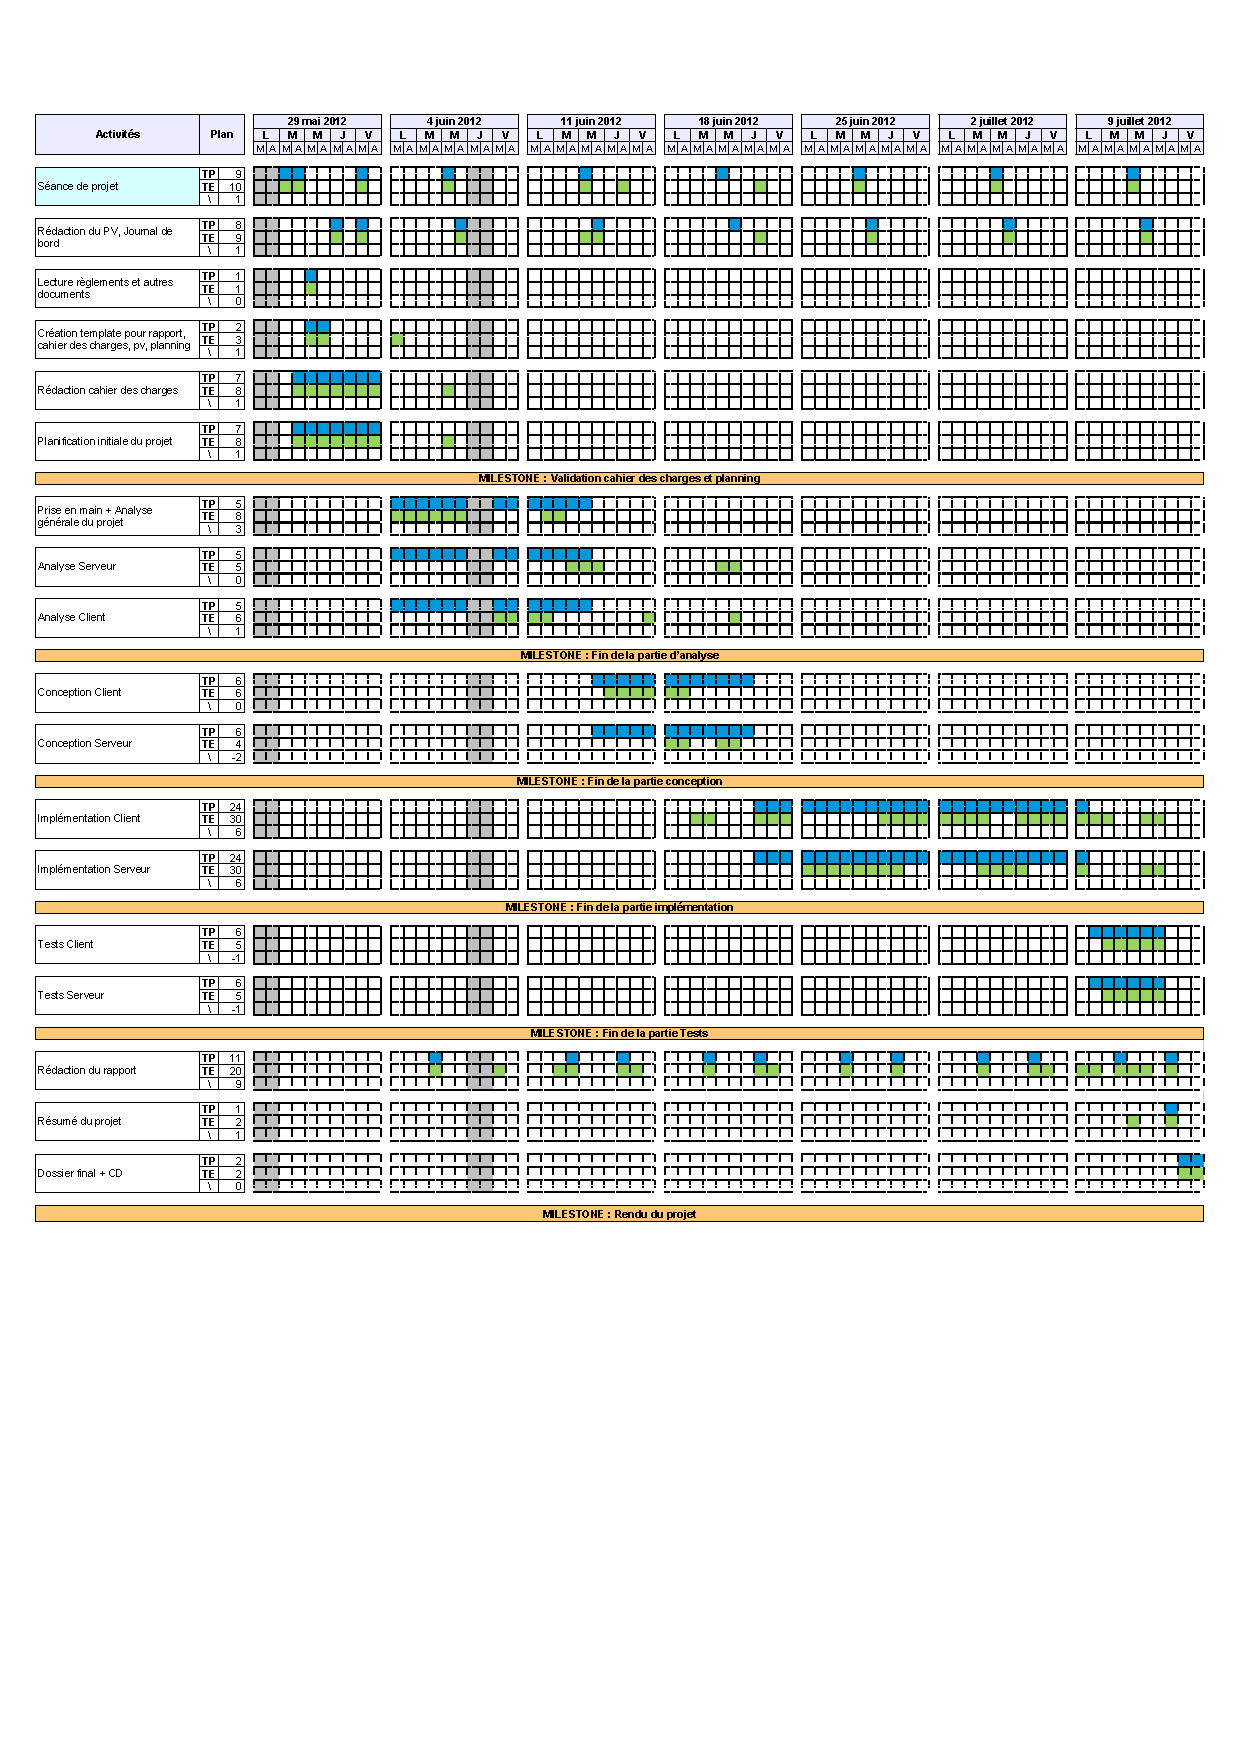
\includegraphics[width=\textwidth]{00_media/00_planning.pdf}
    	\caption{Planning du projet}
    	\label{gra:pla}
\end{figure}
% chapter planning (end)

\chapter{Description de la structure du DVD}
\label{cha:descriptionCD}

\dirtree{%
.1 01\_Cahier\_des\_charges --> contient les versions du cahier des charges.
.2 Sources --> contient les sources latex du cahier des charges.
.1 02\_Rapport --> contient une version du rapport destinée à être lue et une autre destinée à être imprimée.
.2 Sources --> contient les sources latex du rapport.
.1 03\_Planning --> contient toutes les versions du planning.
.1 04\_PV --> contient tous les procès-verbaux des séances.
.2 Sources --> contient les sources latex des pv.
.1 05\_Journal\_de\_bord --> contient le journal de bord.
.1 06\_Workspace --> contient les sources des applications.
.2 client --> contient les sources de l'application cliente.
.2 serveur --> contient les sources de l'application serveur.
}
% chapter proc_s_verbaux (end)